\begin{Exercise}[title=Chute d'un cadre dans un champ magnétique]
Chute d’un cadre dans un champ magnétique Un cadre rectangulaire de résistance $R$
est situé dans un plan vertical. Le cadre est placé dans un champ magnétique$\vec{B}=b\vec{x}$ constant, uniforme et perpendiculaire au plan du cadre. On prend comme origine du temps le dernier instant où le cadre est entièrement plongé dans le champ magnétique
(voir figure). On donne au cadre un mouvement de translation uniforme de vitesse $\vec{v}=-v\vec{z}$ parallèle au coté $AA'=a$
\begin{center}
  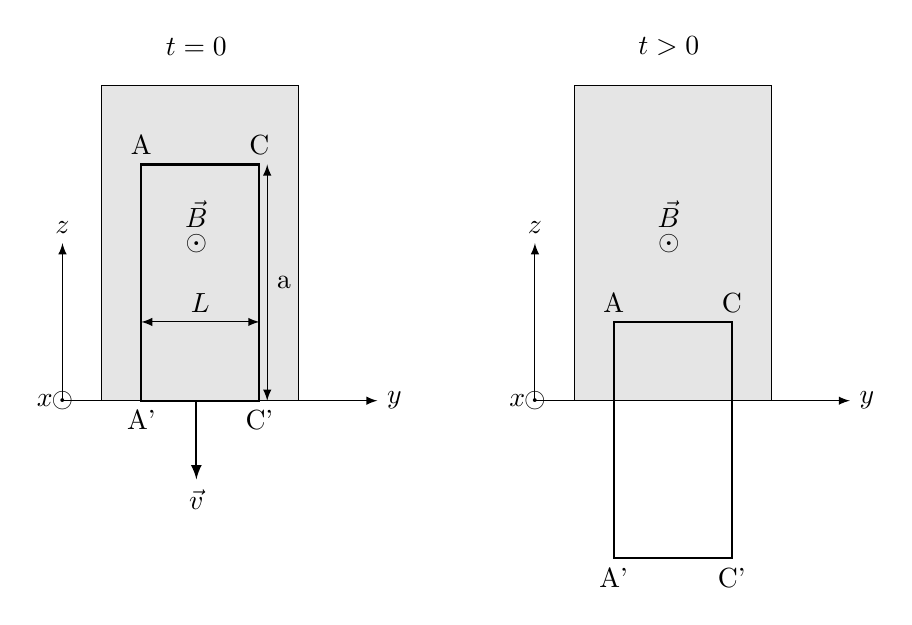
\begin{tikzpicture}
    \begin{scope}
      \draw[-latex] (0,0) -- (4,0) node[right]{$y$};
      \node at(1.7,4.5) {$t=0$};
      \draw[-latex] (0,0) -- (0,2) node[above]{$z$};
      \fill[gray!20,draw] (0.5,0) rectangle (3,4);
      \draw (0.5,0) rectangle (3,4);
      \node (B) at (1.7,2) {$\odot$};
      \node[above=0.2em] at (B) {$\vec{B}$};
      \node (O) at (0,0){$\odot$};
      \node[left] at (O) {$x$};
      \coordinate (A') at (1,0);
      \coordinate (A) at (1,3);
      \coordinate (C) at (2.5,3);
      \coordinate (C') at (2.5,0);
      \draw[thick] (A') rectangle (C);
      \node[above] at (A) {A};
      \node[below] at (A') {A'};
      \node[above] at (C) {C};
      \node[below] at (C') {C'};
      \draw[latex-latex] (C)++(0.1,0) -- ++(0,-3) node[midway, right]{a};
      \draw[latex-latex] (1,1) -- ++(1.5,0) node[midway,above]{$L$};
      \draw[thick,-latex] (1.7,0) -- ++(0,-1) node[below]{$\vec{v}$};
    \end{scope}
    \begin{scope}[shift={(6,0)}]
      \node at (1.7,4.5) {$t>0$};
      \draw[-latex] (0,0) -- (4,0) node[right]{$y$};
      \draw[-latex] (0,0) -- (0,2) node[above]{$z$};
      \fill[gray!20] (0.5,0) rectangle (3,4);
      \node (B) at (1.7,2) {$\odot$};
      \draw (0.5,0) rectangle (3,4);
      \node[above=0.2em] at (B) {$\vec{B}$};
      \node (O) at (0,0){$\odot$};
      \node[left] at (O) {$x$};
      \coordinate (A') at (1,-2);
      \coordinate (A) at (1,1);
      \coordinate (C) at (2.5,1);
      \coordinate (C') at (2.5,-2);
      \draw[thick] (A') rectangle (C);
      \node[above] at (A) {A};
      \node[below] at (A') {A'};
      \node[above] at (C) {C};
      \node[below] at (C') {C'};
    \end{scope}


  \end{tikzpicture}
\end{center}
\Question Calculer la force électromotrice $e(t)$ à partir de la loi de faraday.
\Question Calculer l’intensité du courant $I$ dans le cadre pour $t > 0$. Vérifier que la loi de Lenz est satisfaite.
\Question Calculer la force F a (amplitude et direction) à appliquer pour vaincre les forces magnétiques (i.e. la force appliquée nécessaire pour garder la vitesse constante)
\Question Calculer le travail dépensé pour sortir le cadre du champ. Comparer avec le travail obtenu en utilisant le théorème de Maxwell.
\Question Calculer la puissance dissipée par effet Joule dans le cadre

\Question Calculer l’énergie dissipée par effet Joule. Comparer avec le travail appliqué.
\end{Exercise}
\begin{Answer}
  \Question $e = - \deriv[\phi]{t} = BLv$
  \Question $ i= e/R = vBL/R$ tant qu'une partie du cadre est dans le champ.
  \Question $ \vec{F}=-\vec{f_{l}} = -\int_{C}^{A}i\vec{dl}\wedge\vec{B} = -iBL\vec{z}$ (les autres segment se compense ou nul)
  \Question $W = \int_{0}^{a}(\vec{F_{a}}.\vec{dr}=IBLa=-W_{l}=I\Delta\Phi$
  \Question $P_{J}=RI^{2}=\frac{v^{2}B^{2}L^{2}}{R}$
  \Question $W_{J}=\int_{0}^{t_{f}}P(t)\d t= IBLa $
Le frein de laplace dissipe l'énergie sous forme de chaleur.
\end{Answer}
